\documentclass{scrartcl}

% packages
\usepackage{amsmath}
\usepackage{amssymb}
\usepackage[ngerman]{babel}
\usepackage{booktabs}
\usepackage[font=small,labelfont=bf]{caption}
\usepackage{csquotes}
\usepackage{float}
\usepackage{fontspec}
  \setmainfont[Ligatures=TeX]{Tex Gyre Pagella}
\usepackage{graphicx}
\usepackage[pdfusetitle,unicode]{hyperref}
\usepackage{mathtools}
\usepackage{microtype}
\usepackage{siunitx}
  \sisetup{separate-uncertainty=true}
\usepackage{subcaption}
\usepackage[math-style=ISO,bold-style=ISO]{unicode-math}
  \setmathfont{Tex Gyre Pagella Math}
\usepackage{xfrac}

% options
\setlength{\parindent}{0pt}  % no stupid indentation

% commands
\DeclarePairedDelimiter{\abs}{\lvert}{\rvert}
\DeclarePairedDelimiter{\mean}{\langle}{\rangle}
\renewcommand{\vec}[1]{\mathbf{#1}}
\renewcommand{\i}{\mathrm{i}}
\DeclareRobustCommand{\e}{\ensuremath{\mathrm{e}}}

% meta
\author{Kevin Dungs \and Kevin Heinicke \and Holger Stevens}
\title{Computational Physics}
\subtitle{Übungsblatt 5}

% document
\begin{document}
\maketitle

\section*{Hausaufgabe 11: MC Simulation des 2-D Ising-Modells (Teil 1)}
Wir wählen periodische Randbedingungen für alle Aufgabenteile.

\paragraph{(a)} In \autoref{fig:equi} ist für verschiedene Werte von $k_BT$ die Energie des Systems gegen die Schrittzahl des Metropolisalgorithmus aufgetragen. Daraus lässt sich schließen, dass ein Burn-In von ca. \num{1e8} Schritten notwendig ist. Die dazugehörigen Werte werden von der Funktion \texttt{runMetropolisAndSaveResults} in \texttt{ising.cc} berechnet.

\begin{figure}[H]
    \centering
    \begin{subfigure}{.32\textwidth}
        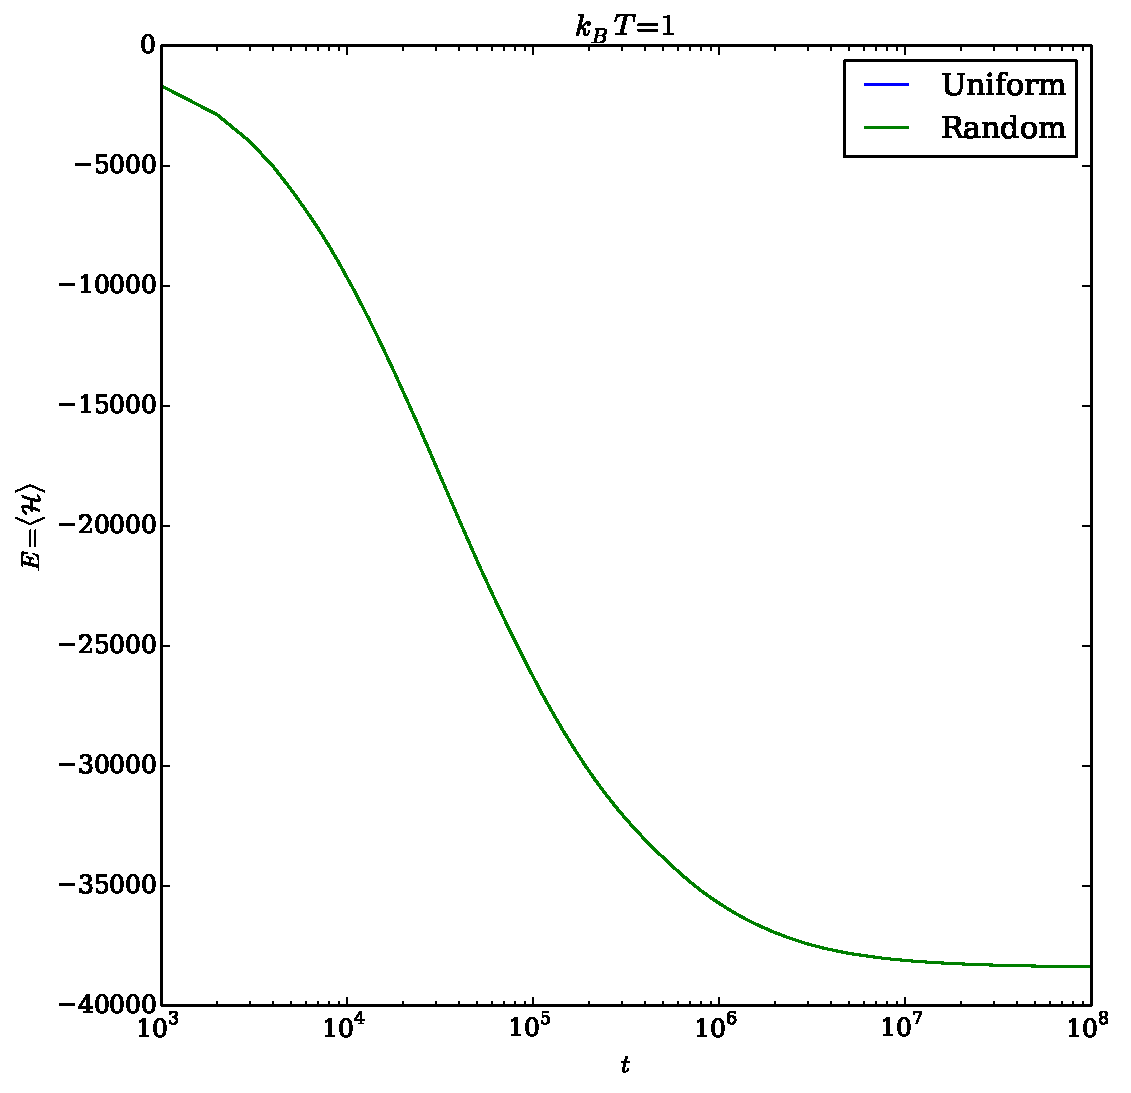
\includegraphics[width=\textwidth]{plots/1.pdf}
        \caption{$k_BT = 1$}
    \end{subfigure}%
    \begin{subfigure}{.32\textwidth}
        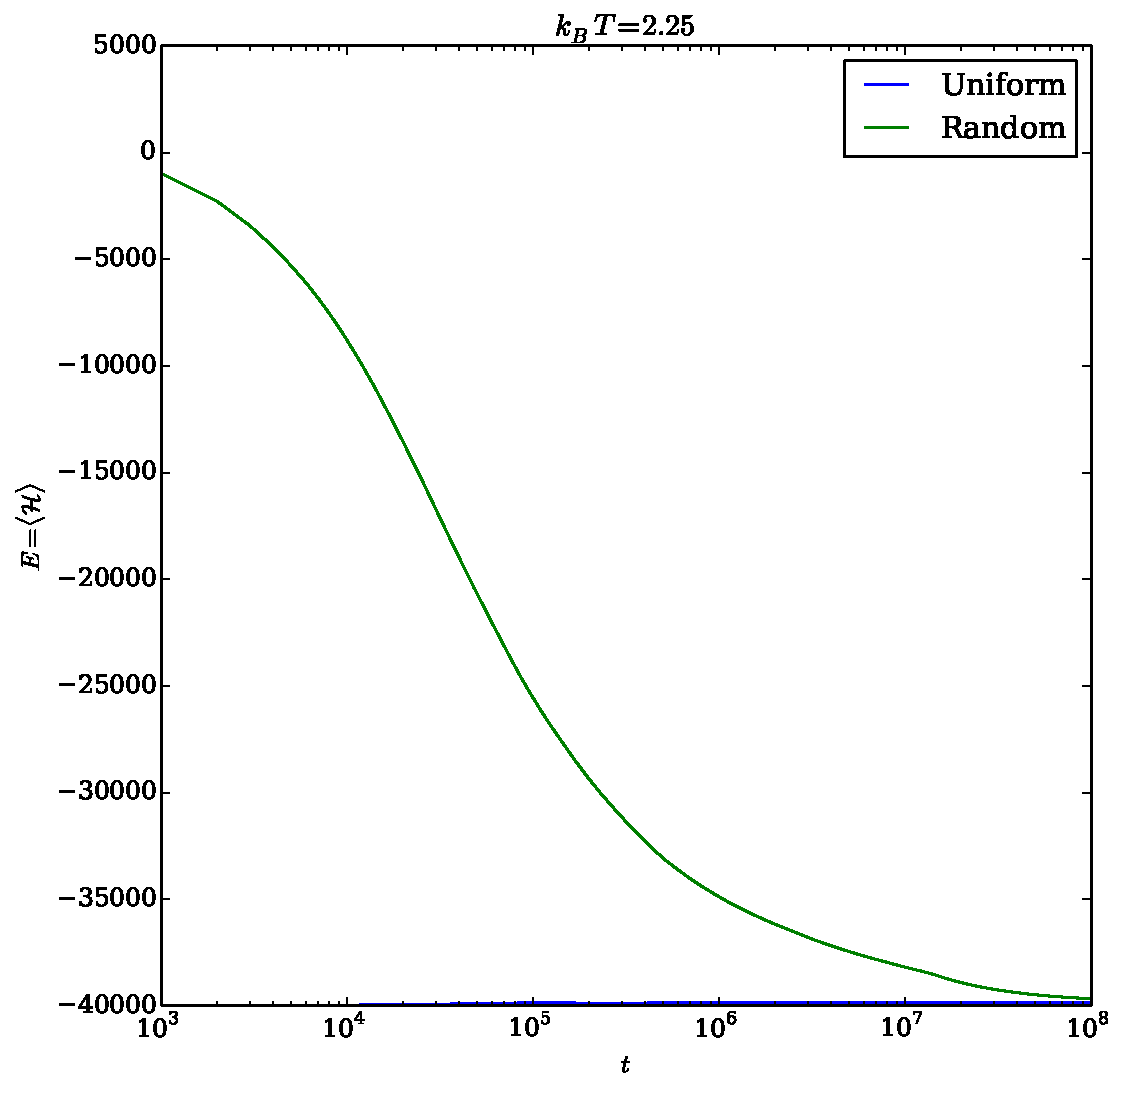
\includegraphics[width=\textwidth]{plots/2_25.pdf}
        \caption{$k_BT = 2.25$}
    \end{subfigure}%
    \begin{subfigure}{.32\textwidth}
        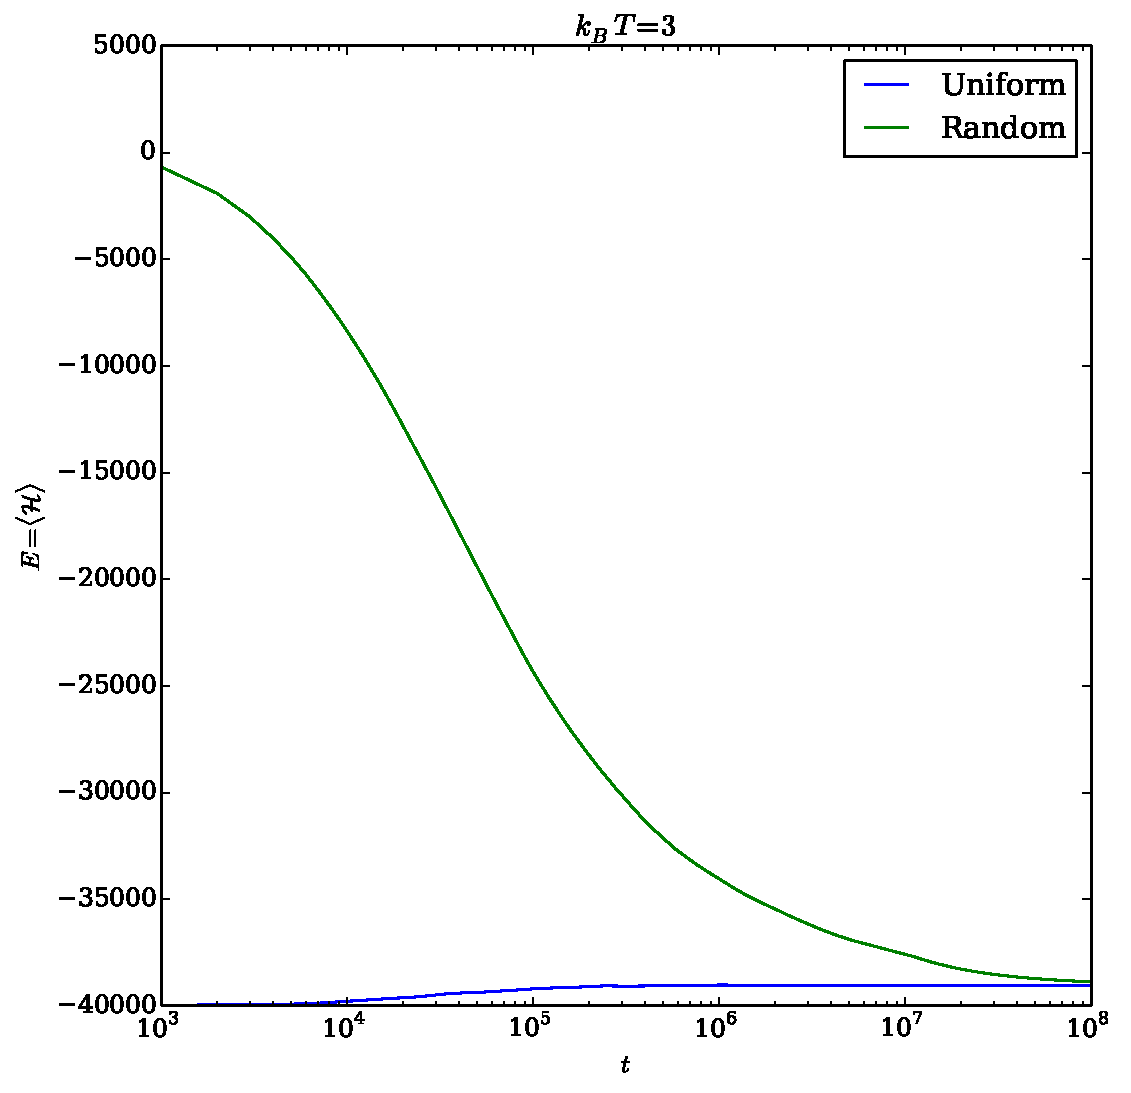
\includegraphics[width=\textwidth]{plots/3.pdf}
        \caption{$k_BT = 3$}
    \end{subfigure}
    \caption{Energie in Abhängigkeit des Algorithmusschrittes.}
    \label{fig:equi}
\end{figure}

\paragraph{(b)} Die Funktion \texttt{runMetropolisAndSaveResults} speichert außerdem die letzte Konfiguration des Systems in einer Textdatei. Die Konfigurationen sind für die verschiedenen Werte von $k_BT$ in \autoref{fig:conf} abgebildet. Dabei ist zu beobachten, dass mit steigender Temperatur weniger große Cluster auftreten.

\begin{figure}[H]
    \centering
    \begin{subfigure}{.32\textwidth}
        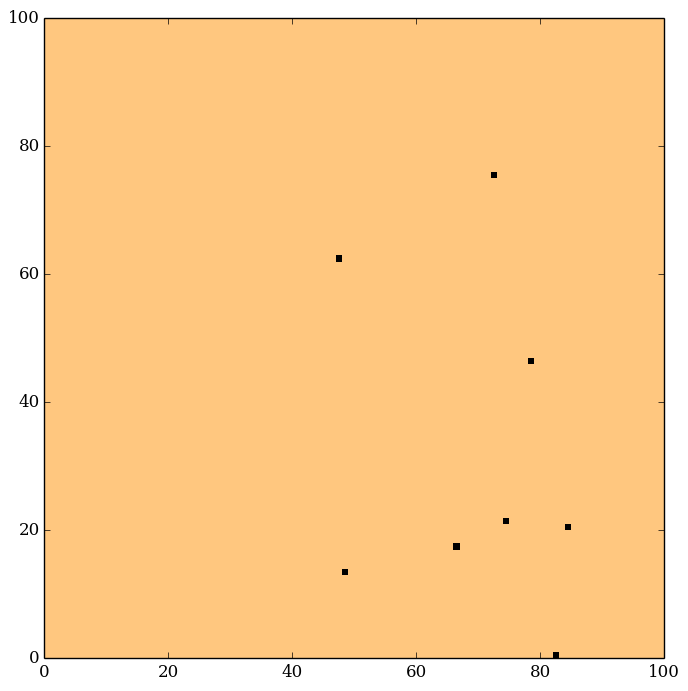
\includegraphics[width=\textwidth]{plots/sc_u_1.png}
        \caption{$k_BT = 1$}
    \end{subfigure}%
    \begin{subfigure}{.32\textwidth}
        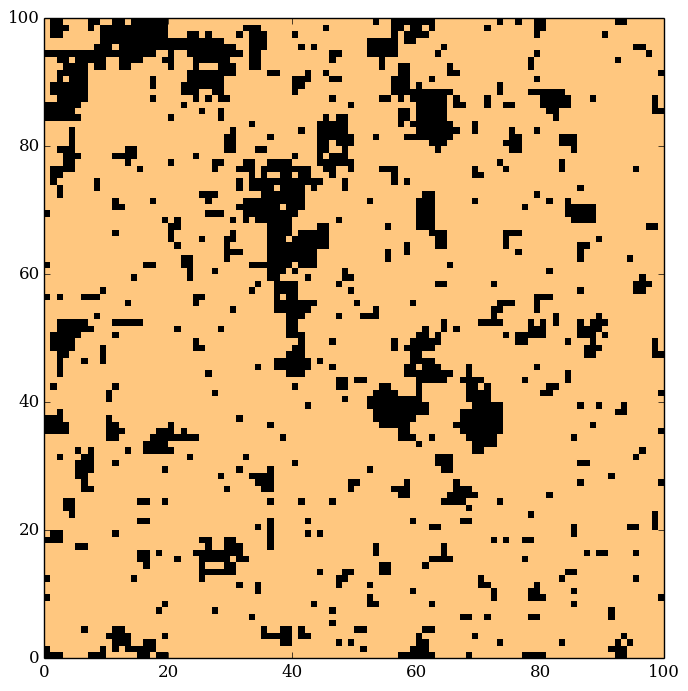
\includegraphics[width=\textwidth]{plots/sc_u_2_25.png}
        \caption{$k_BT = 2.25$}
    \end{subfigure}%
    \begin{subfigure}{.32\textwidth}
        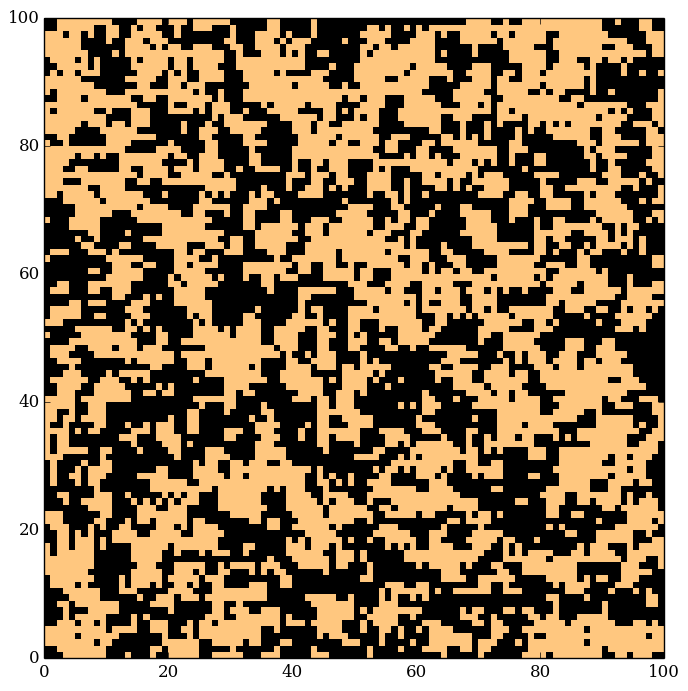
\includegraphics[width=\textwidth]{plots/sc_u_3.png}
        \caption{$k_BT = 3$}
    \end{subfigure}
    \begin{subfigure}{.32\textwidth}
        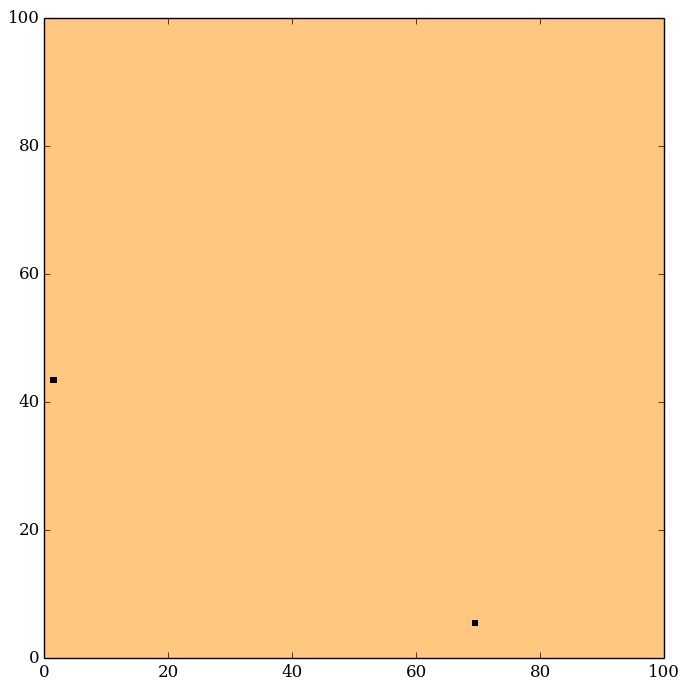
\includegraphics[width=\textwidth]{plots/sc_r_1.png}
        \caption{$k_BT = 1$}
    \end{subfigure}%
    \begin{subfigure}{.32\textwidth}
        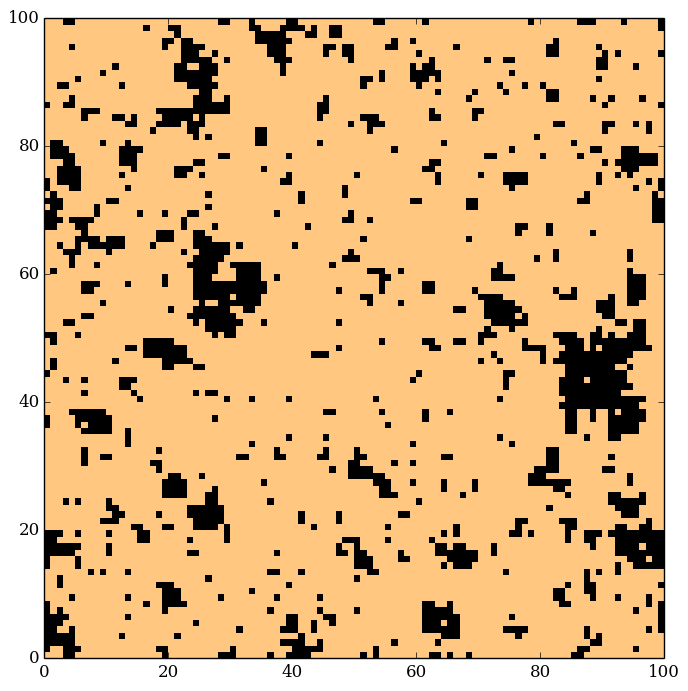
\includegraphics[width=\textwidth]{plots/sc_r_2_25.png}
        \caption{$k_BT = 2.25$}
    \end{subfigure}%
    \begin{subfigure}{.32\textwidth}
        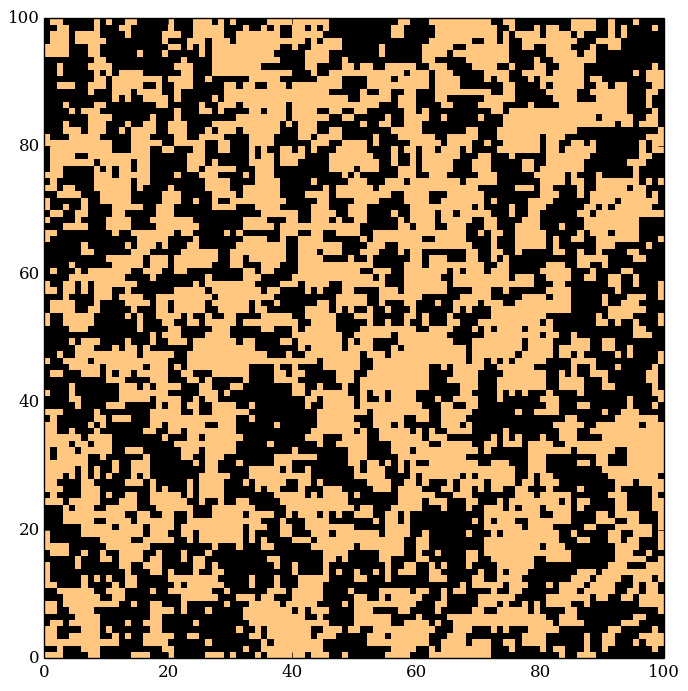
\includegraphics[width=\textwidth]{plots/sc_r_3.png}
        \caption{$k_BT = 3$}
    \end{subfigure}
    \caption{Konfiguration des Systems nach \num{1e8} Schritten. Spins up sind in orange, Spins down in schwarz dargestellt. In der oberen Reihe sind die Ergebnisse bei uniformer Anfangskonfiguration und in der unteren Reihe die bei zufälliger Anfangskonfiguration (\SI{50}{\percent} up, \SI{50}{\percent} down) abgebildet.}
    \label{fig:conf}
\end{figure}

\paragraph{(c)} Die Funktion \texttt{metropolisMeasureEnergyAndSaveConfiguration} in \texttt{ising.cc} berechnet nach einer Burn-In-Phase von \num{1e8} Schritten die gemittelte Energie $E_{\text{Metropolis}}$ aus \num{1e4} Schritten, der angegebene Fehler ist also der Fehler des Mittelwertes. Dabei ist $J_x = 1$ und $J_y = 0$ sowie $\beta = 1$. Der analytische Wert berechnet sich nach länglicher Umformung und Grenzwertbetrachtung zu $E_{\text{Analytisch}}$. In \autoref{fig:decoupled} ist eine Momentaufnahme des Systems dargestellt.

\begin{align*}
    E_{\text{Metropolis}} &= \num{-7604.1 \pm 0.2} \\
    E_{\text{Analytisch}} &\approx -N\frac{\sinh\beta J}{\cosh\beta J} = \num{-7615.9} \\
\end{align*}

\begin{figure}[H]
    \centering
    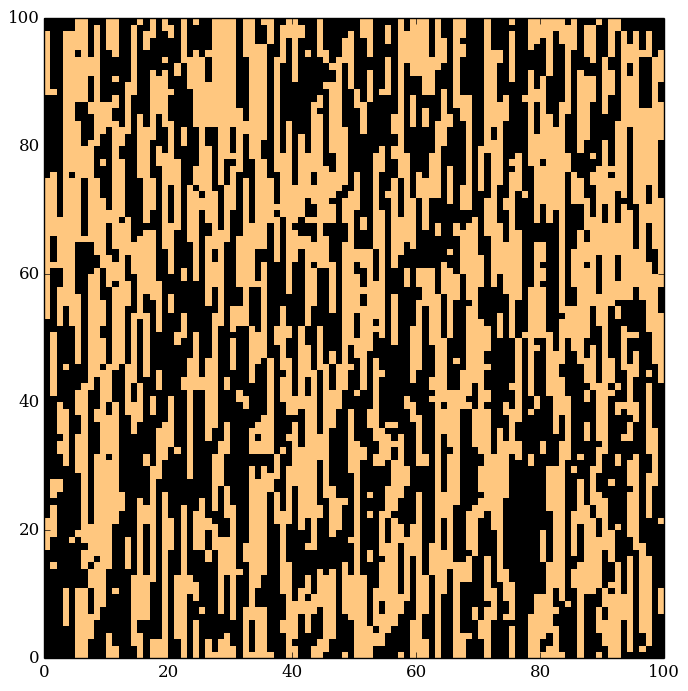
\includegraphics[width=.5\textwidth]{plots/decoupled.png}
    \caption{Momentaufnahme des entkoppelten Systems. Es ist deutlich zu sehen, dass sich in vertikaler Richtung Cluster ausbilden.}
    \label{fig:decoupled}
\end{figure}

\end{document}
